\chapter{Technical Design Development}

\section{Organisational Breakdown Structure}
In order to optimise technical development, the team has identified critical, non-technical responsibilities and distributed them amongst its members, as shown in \autoref{fig:organogram}. The aim of these roles is to provide a structure to technical development, mitigating internal developmental risks and increasing the overall quality of the final product. The roles identified, and their description, are as follows:

\begin{itemize}
    \item Chairman: Responsible for guiding group meetings and discussions. Prepares meeting agendas and ensures conversations stay relevant to the team goal.
    \item Secretary: Responsible for documenting meetings. Main point of contact with all external stakeholders.
    \item Project Management: Maintains an oversight of the entire project, ensuring appropriate progression in relation to upcoming deadlines.
    \item Systems Engineering: 
    \item Documentation:
    \item CAD:
    \item Sustainability:
    \item Quality Assurance:
    \item Git:
\end{itemize}

\begin{figure}[h]
    \centering
    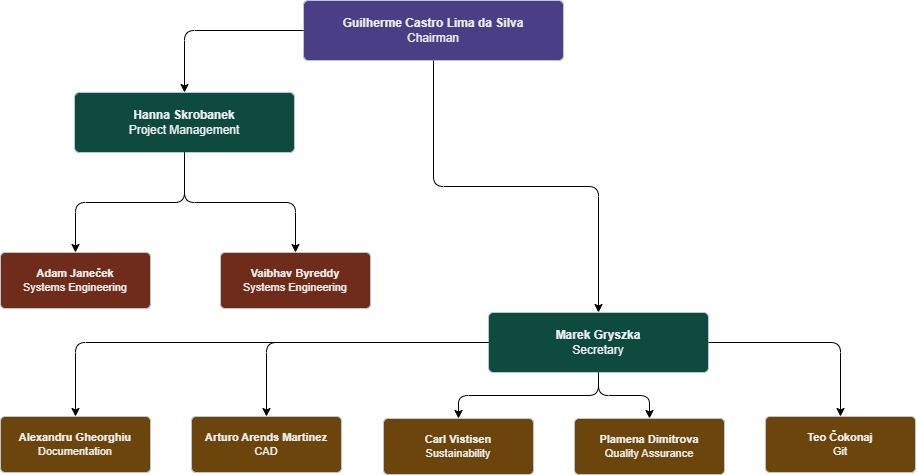
\includegraphics[width=\linewidth]{figures/Group 28 Organigram.jpg}
    \caption{Organogram detailing the organisational structure of Group 28}
    \label{fig:organogram}
\end{figure}

\section{Team technical roles}
According to the project guide \cite{}, where the percentages of relevant technical expertise required for the project are stated, the team is divided into several sub-groups based on the technical expertise of the members. The technical expertise groups were labeled \textbf{AERO}, representing aerodynamics, performance and propulsion, \textbf{ASM}, representing materials and manufacturing, and \textbf{CONTROL}, representing control engineering and systems engineering, and \textbf{OPS}, representing operations. Besides the roles assigned in \autoref{fig:organogram}. The preferences of each team member are presented in \autoref{tab:technical_prefs}.

\begin{table}[H]
    \centering
    \begin{tabular}{|c|c|}
         \hline
         \textbf{Group member} & \textbf{Technical expertise} \\
         \hline
         Adam &  AERO, CONTROL, OPS\\
         \hline
         Alex &  CONTROL\\
         \hline
         Arturo &  ASM\\
         \hline
         Carl &  AERO\\
         \hline
         Guilherme &  CONTROL\\
         \hline
         Hanna &  ASM\\
         \hline
         Marek &  ASM\\
         \hline
         Plamena &  AERO\\
         \hline
         Teo &  CONTROL, ASM\\
         \hline
         Vaibhav &  ASM, AERO\\
         \hline
    \end{tabular}
    \caption{Caption}
    \label{tab:technical_prefs}
\end{table}